\chapter{State of Art}
\section{Smart Home Research}
\subsection{Overview}
The smart home system we discussed about, that is also described as automated home, integrated home systems or intelligent building\cite{smart_home_concept}, has drawn more and more industry developers' and researchers' attention over the decades, research groups such as Siemens, IBM, Cisco, Microsoft\cite{smart_home_research} has already contributed in this domain. A great number of Smart Home application, network protocols as well as gateways\cite{smart_home_for_gateway} have come into world and been applied to benefit their customers.

With the development of Smart Home technology, nowadays' Smart Home is not only in charge of monitoring and controlling lighting and heating inside the building, but also capable of connecting almost every electronic devices, inhabitant action prediction as well as making scheduler decisions. Functionalities provided by intelligent home are not just limited to turn device on and off, record and report senor data, but include self-adjusting the inner building environment, supporting various predefined patterns, such as energy saving pattern, especially the concept of Smart Home for elderly\cite{smart_home_for_old}, which perfectly combines modern remote control and monitoring technologies, with senior-friendly and patient-concerning housing, is welcomed by the market. 

Three categories of Smart Home will be introduced in the following as best practice examples, they are Smart Home optimized for energy services , Smart Health Home and Agent-based Smart Home.
 
\subsection{Smart Home Optimized for Energy Services}
This type of Smart Home put its main goal in the energy saving and monitoring domain, which helps householder to make wiser decisions under the energy crisis background. 

The key component in this Smart Home is decision-support tool\cite{smart_home_for_energy}, that applies a scheduling algorithm which offers house owner suggestion based on various parameters such as distributed energy resources(DER), with the prospect of energy and resource saving.

\subsubsection{Decision Support Tool}

 \begin{figure}[!htbp]
	\centering
	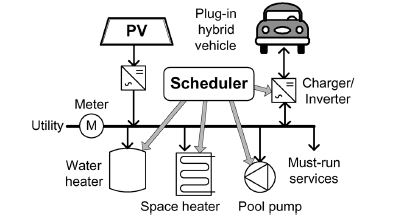
\includegraphics[width=1.0\textwidth]{scheduler.jpg}
		\caption{DER Scheduler in Smart Home optimized for energy\cite{smart_home_for_energy}}
	\label{fig:smart-home-scheduler}
\end{figure}

The decision support tool used in paper\cite{smart_home_for_energy} consists of two components, they are energy service model which describes the energy service request and distributed energy resource scheduling algorithm, as described in figure~\ref{fig:smart-home-scheduler}. To be more specifically, energy service model presents the demand for one particular energy resource. For instance the demand aimed at hot water means, the hourly consumption of heated water or the energy that is hourly needed by water heater.  According to \cite{smart_home_for_energy}, the heat content of water is also defined as "energy equivalent" and therefore the energy service model is applied to increase "monetary benefit"  from every "energy equivalent" unit.

Meanwhile the DER scheduler algorithm helps householder by reducing the unnecessary consumption of energy. This algorithm is in nature one mathematical optimization problem defined by\cite{smart_home_for_energy}.
\begin{center}
 $ \sum_{t=1}^{T}\sum_{i=1}^{S}[\lambda_{ES,i}(t)\cdot {U_{ES,i}}(t,x)]-Cost$
\end{center}

The purpose of DER scheduler, presented as \emph{x} is to maximize that above introduced fitness function, where \emph{S} represents all number of services offered by Smart Home, \emph{T} stands for the whole simulation time, $\lambda_{ES,i}$ and $ U_{ES,i}$ describe the desired monetary benefit for "energy equivalent" and energy demand of the \emph{i}th service respectively. \emph{Cost} means the total electricity consumption. Also in paper\cite{smart_home_for_energy} the choice of DER algorithm is well discussed.


\subsection{Smart Health Home}
Another suitable application domain for Smart Home is the Smart Health Home, which describes the intelligent housing that takes care of patients at home or elder residents.

The charming features of this Smart Home system are the combination of telemedical system with communication technologies\cite and customizing services such as, teleconsulting, telediagnosis, real time imaging as well as distance medical education\cite{smart_home_for_health}, which together improve the living condition of householder and at the same time build a caring system that takes care of residents' need. Nine best practice examples are provided and evaluated in paper\cite{smart_home_for_old}, they provide a guideline for  the design of Smart  Home system and summarizes precio

us experience. 
 \begin{figure}[!htbp]
	\centering
	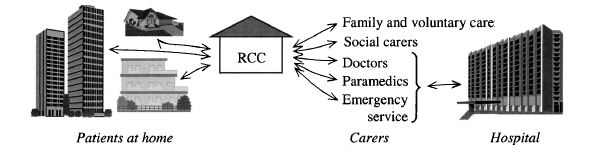
\includegraphics[width=1.0\textwidth]{rcc.jpg}
		\caption{Overview of Smart Health Home structure\cite{smart_home_for_health} (RCC: Remote Control Center)}
	\label{fig:rcc}
\end{figure}
\subsection{Agent-based Smart Home}
Agent-based Smart Home aims to build an intelligent home that based on machine learning, artificial intelligence technology and mobile computing predicts householders' behaviors, makes appropriate decisions. The achieved prediction can help residents to experience more comfortable and convenience living condition. MavHome ( Managing An Intelligent Versatile Home)\cite{smart_home_agent} builds the best example. 

\subsubsection{MavHome architecture}
 \begin{figure}[!htbp]
	\centering
	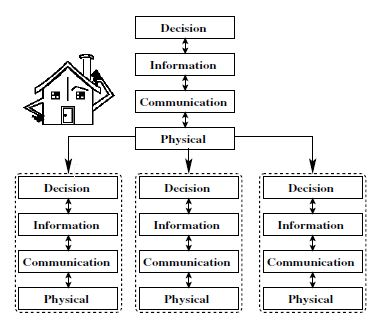
\includegraphics[width=0.8\textwidth]{smart-home-agent.jpg}
		\caption{MavHome agent architecture\cite{smart_home_agent}}
	\label{fig:smart-home-agent}

\end{figure}
As shown in figure~\ref{fig:smart-home-agent}, agents which are employed by MavHome consist of four different layers. From bottom to top:
\begin{itemize}
\item \emph{Physical layer}, where hardwares that together build Smart Home system are deployed. Moreover, underlaying agents can also act as physical layer for other agents.
\item \emph{Communication layer}, this layer provides communication services for agent by using functionalities offered by physical layer.
\item \emph{Information layer}, as higher layer of Smart Home system,  the responsibilities for this layers are gathering and maintaining information which is used by decision layer.
\item \emph{Decision layer}, in this layer agents make decision as well as learn resident's preference and correct the unwanted system behavior.
\end{itemize}
\subsubsection{Prediction algorithm}
Prediction algorithm is the core component of MavHome project. Several Strategies are presented on the first IEEE international conference on pervasive computes and communication, they are SHIP algorithm that is based on sequence matching, compression-based prediction algorithm ALZ and Task-based Markov model\cite{smart_home_agent}.

\subsection{Conclusion}
Also described above, Smart Home is the representative application which is based on industrial automation, remote control, management and coordination system. Despite the decision making algorithms and application level components from above mentioned smart buildings are different from the other, but they all are integrated upon or connected with housing devices. The management and cooperation with those devices must take place under a secure system environment. None of householders are willing to be monitored by a strange third party using his own camera or to expose their daily life related information to public. Therefore one common request for the design of such intelligent building is to ensure the system security.

Based on the fact, that home devices applied by Smart Home are manufactured by various vendors,  Smart Home designers also must take it into account, that how to realize the system interoperability. Considered those two requirements, the idea of this thesis applying OPC UA standards with smart card technology came into world. 

\section{OPC UA Application and Security policy }

\subsection{OPC UA applications}
OPC UA, as explained in former paragraphs,  is understood as a platform independent, well designed, secure concerned, IEC standard compliant, promising industry standards set, which provides a service oriented architecture and is being widely applied in industry application such as critical control system and industrial automation. Application examples are given in following paragraphs, each of which has different focus. To be more specifically, the charming demonstrated characteristics of OPU UA standard set are: secure consideration, real time data exchange and management, scalability. 

\subsubsection{OPC UA and ICS}
With develop of industrial automation, Industrial control system (ICS) has became a hot topic, but most manufactures putted much more effort in designing automation and manufacturing process and neglected the communication security issues. As a consequence, Cyber security of ICS now is drawing more and more attentions from industry. OPC UA offers manufactures who are applying ICS system not only object oriented modeling rules, which can be extremely helpful for developers that design domain specific model and manufacturing process, but also provides them a reliable and robust security model\cite{opc_ics}, that has various secure arrangements in each communication protocol stack layer.


\subsubsection{OPC UA and  Smart Grid}
Smart Grid is now concerned as the future of electricity energy industry and therefor how to achieve an intelligent electricity distribution as well as behavior coordination between customs and suppliers is a hot topic\cite{opc_grid}. Electricity industry is searching out for a standardized communication technology to solve aforementioned issue.
OPC UA standards set that includes \emph{alarm and even} model, \emph{data access} model as well as  \emph{historical data access} model, is without doubt one the of best candidates. With the help of all these models, the secure real-time communication and stockholders' coordination are guaranteed.

\subsubsection{Nano OPC UA }
Apart from those enterprise level systems, OPC UA is also suitable for lower level field devices, such as field sensor and other resource limited facilities. Recently a German company Lemgo even designed a nano embedded OPC UA server\cite{opc_lemgo}, which provides the core OPC UA server service set. adopts TCP binary communication protocol and is implemented on a chip device.

\subsection{OPC UA secure policies}
At the design beginning, the OPC foundation has taken the construction of secure and robust communication protocol as the center and therefore developed a enhanced consistent security model which has clear and definite objectives in each layer of OPC UA transport and communication stack. In present day, OPC UA  offers secure messaging mechanisms by applying WS Security with Simple Object Access Protocol (SOAP)  and alternatively SSL based Hypertext transfer Protocol Secure (HTTPS) messaging\cite{opc_secure_1}. Besides secure messaging protocols,  authentication mechanisms based on username-password or X.509 certificates are introduced, in order to process mutual authentication among OPC UA applications from different logic levels and hardware devices.

OPC foundation uses the term \emph{secure policies}\cite{O2} to describe the 
user authentication, user authorization and application authentication mechanisms proposed by one OPC UA server profile. In this server profile, both secure related requirements and other server functionalities are described. One server is capable of maintaining several profiles in order to provides services to different clients, who might have various demands for security. Meanwhile one client can also accept a list of profiles, each of them is assigned by one server with particular security objectives. 

\subsection{OPC UA design consideration}
Along with core services set including data read and write services, notification service etc., OPC UA server also provides \emph{discover service}\cite{O4}, which provides OPC UA clients mechanism to require server secure policy, and \emph{secure channel service} set\cite{O4}, that is used to create and management secure channel with acknowledgment such as key deviation algorithm and encryption algorithm achieved from secure policy. 

Also OPC UA specifications provide guide lines for a secure system design\cite{O4}.
\begin{itemize}
\item \emph{appropriate timeout} Timeout mechanism is widely employed in systems that adopt client server architecture. With reasonable configured timeout property, both client and server can avoid unnecessary resource consumption by long time waiting response from the other, which could be caused by unexpected physical device failure or intentionally server denial of service attack initiated by third party and etc. 
\item \emph{rate control} Rate control is considered as one of the most practical approach to prevent denial of service attack. Under rate control mechanism, each client has limited chance over a period to build communication channel, reconstruct this channel, require information from server or send data to sever. Alternatively server can also ban or block the client for a period of time, who is recently trying to flood messages. 
\item \emph{random number generation} The generation of random number is required by most encryption, authentication and authorization algorithms. Therefore a secure system must support robust random number generation.s
\item \emph{strict message processing}, which means the exchanged message between two communication partners must be compliant with predefined message format. Any ill-formed messages must be ignored, which in turn helps to avoid stack overflow attack and enhances system security
\item \emph{historical data management}, this strategy ensures the system traceability and records any behaviors taking place in system. And the recorded data can be used for forensic research, when security related issues happens.
\end{itemize}
\subsection{Conclusion}
Above pictured OPC UA standards' features and characteristics prove the feasibility of applying OPC UA as communication protocol for Smart Home proposed in this thesis.

\section{Smart Card Security}
Integrated circuit cards, ICCs for short, was firstly designed and patented in Germany\cite{smart_card_history}. Since then this credit size-, embedded with circuit chip- card is being applied in more and more various industry domains, such as secure information storage media, on-line access token, identification method, small amount payment mechanism and etc. With the development of smart card technologies, nowadays apart from traditional \emph{contact smart card}, \emph{contactless smart card}\cite{smart_card_contactless} has come into market. This \emph{contactless smart card} is able to communication with card access device without direct physical connection. To be more precisely, it applies radio frequency to contact with CADs. Now matter what categories of smart card, the temper resistant nature always contributes to make them to be one of the most popular secure token medias.
\subsection{Smart Card in Access Control}
In present days, \emph{security} no longer just meant the secure of our homeland borders, or the individual personal safety. In this information age, the word \emph{security} also refers to the confidentiality and integrity of users' personal data, the robustness of information system and so on. It is immediately concerned with our daily life. Especially when electronic devices, which can carry sensitive and precious information and could be vulnerable to malicious attackers, are playing irreplaceable roles in our society. 

Smart card, as explained in section \emph{fundamental technologies}, is believed as one of the best secure mechanism for access control and user identification. There three ways to identity a person\cite{handbuch}:
\begin{itemize}
\item \emph{1 knowledge about a secret}, the secret is normally a password that negotiated early between two identification peers.
\item \emph{2 possession of an object}, this object could be anything that is predefined. One example could be the open door keys.s
\item \emph{3 biometrics identification}. First two points have their own limitations, because third part could steal the object, that is used for identification, or copy user's password. Moreover it also can happen, that password too long or too complex to remember or identification object is hard to carry with. Compared with them, biometrics identification depends on however the human body characteristics, such as fingerprint, signature and retina recognition.
\end{itemize}
Based on the above described facts, smart card is the best candidate for user identification and access control. Because when anyone wants to perform identification using smart card, he must possess the card (possession of an object satisfied), input PIN to unlock and to access card (knowledge about a secret). At the same time, complex passwords for the purpose of peer authentication and authorization can be stored on the smart card, which helps card holder to release the burden of remembering them. Also on same cards there exits a signature signed by card holder or a card holder photo, that could be use to perform biometrics identification. 

Nowadays with the help of standards such as \emph{GPC\_2.2\_B\_RAM\_over\_HTTP}, which is introduced in section \emph{fundamental technologies}, smart card is also capable of performing on-line identification based on either certificate or TLS protocol.

\subsubsection{Personal Identification Number}
Whenever an user intends to use one smart card, he must input a \emph{personal Identification Number}, which is also referred as \emph{Card Holder Verification}. PIN consists usually of four decimal number from 0 to 9 and tolerates at most 3 times wrong PIN input before a successful verification. PIN is usually stored in elementary files\cite{smart_card_access} on smart card in order to be kept from unauthorized modification. After 3 times wrong PIN input, a smart card will be locked until the \emph{unlock PIN} operation is successfully carried out. Moreover if \emph{unlock PIN} operation also fails three times in a roll, the PIN will never be unblocked\cite{smart_card_access}.

\subsection{Key Management}

 \begin{figure}[!htbp]
	\centering
	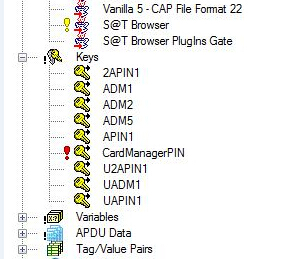
\includegraphics[width=0.45\textwidth]{smart-card-key.jpg}
		\caption{keys presented in Smart Card Description Language from \emph{Morpho}}
	\label{fig:smart-card-key}
\end{figure}

The above introduce PIN is not the only key that are stored on smart card. In order to perform message encryption as well as decryption, peer authentication and etc. smart card must keep various keys in storage. As shown in figure~\ref{fig:smart-card-key}, in one \emph{Morpho} smart card product, a list of keys and key sets are used, for example, Card Manager PIN and Administrative keys (\emph{ADM1, ADM2, ADM5}).

Moreover key data in smart not only simply record the actual key value but also must provide information such as key version number, the usage of key and so on. Table~\ref{table:smart-card-key} describes a typical key data on smart card. Likely the usage of a key also need more than just give  actual key value as shown in figure~\ref{fig:smart-card-key-use}

 \begin{figure}[!htbp]
	\centering
	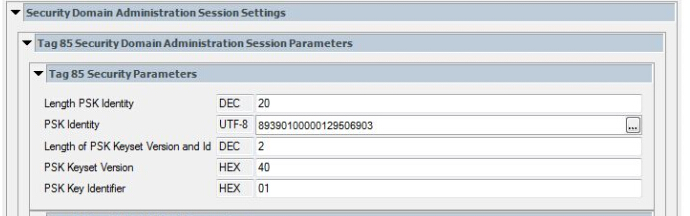
\includegraphics[width=0.85\textwidth]{smart-card-key-use.jpg}
		\caption{the PSK key used to configure administration session}
	\label{fig:smart-card-key-use}
\end{figure}

\begin{table}[!htbp]
\caption{key data stored in smart card\cite{handbook}}
\begin{tabular}{lllll}
\hline\hline
Data object & Remarks\\[0.5ex]
Key number & unique key reference number\\
Version number & version number used for key derivation\\
Intended usage & for which purpose this key is introduced\\
Blocked & used to block a key\\
Retry counter & wrong key input counter\\
Maximum retry count & key will be blocked if retry counter reaches this value\\
Key size & the size of key\\
Key & Key value\\
\hline
\end{tabular}
\label{table:smart-card-key}
\end{table}

Since different keys play distinguished roles in various system tasks and smart card must handle a huge number of keys, \emph{key management} shows its importance. The core responsibilities of key management is listed as following\cite{handbook}:
\begin{itemize}
\item \emph{key generation} Key generation is the initial step of key life cycles and uses usually physical random numbers as initial data, in order to generate secure and unique keys. 
\item \emph{key update} This process keeps one key from being used for a long period, which could lead to compromise of system security.
\item \emph{key revocation} When one key turns out to be compromise, key management system must destruct that key.
\item \emph{key storage} Apparently a competent key management system must know how to safely store its secret.
\end{itemize}
\subsubsection{Key Generation}
\paragraph{Derived Key}
Since smart card can be easily exposed and analyzed by anyone who holds or steals the card, in order to minimize the risk of key compromising, none master keys are present in smart card. As a consequence, keys used in smart card are derived from unique card number, which is given during the card production process, with the help of triple DES and AES cryptographic algorithms\cite{handbook}.
\paragraph{Dynamic Key}
Dynamic key is normally applied to secure communication between peers and therefore it is also known as session key or temporary key. The generation of dynamic keys begins with generation of a random number that is proposed by one communication partner or unique data which is able to specify one particular session. The rest process may be different and let's take \emph{ANSI X 9.17} standard as an example\cite{handbook}. 
\begin{center}
$Key_{i+1} = e(Key_{gen},e(Key_{gen},(T_{i} XOR Key_{i})))$
\end{center}
This process described above is one-way process and can not be reserved. To be more specifically, $T_{i}$ and  $Key_{gen}$ are time-,session-independent initialization input parameter and Key generation key respectively. The newly generated  key $key_{i}$ can not only be used for encryption but also to generate other new keys.
\subsection{Threaten and countermeasures}
In this section, potential smart card vulnerabilities, threatens aimed at chip card as well as countermeasures will be discussed. But before we begin the analysis of smart card threatens, the trust environment of smart card based system should be explained. Following five parties are listed\cite{smart_card_attack1}.
\begin{itemize}
\item \emph{Cardholder} In other word, the owner of smart card, who as customer daily users smart card for different purpose  in various systems. For instance, using SIM card in cell phone to make phone call or using smart card digital wallet to perform smart amount payment like paying the park fee.
\item \emph{Terminal} The card access device that communicates with smart card through smart card I/O.
\item \emph{Card Manufacturer} As the name indicates, card manufacturer is the one who manufactures  the card.
\item \emph{Card Issuer} Card Issuer is the party that designs the card OS and initializes the smart card. For example, if we are taking about a cell phone smart card, then card issuer will be the phone company. When it comes to employees' ID cards which as applied as access control tool for a particular company, in this situation card issuer is the employer.
\item \emph{Software manufacturer} This party is the one who designs applications that run on smart card.
\end{itemize}
\subsubsection{Smart card Threatens and vulnerabilities}
Since threat modeling for smart card could be extreme complex and also the classification of smart card is various. In this paragraph four representative threaten categories are presented. They are\cite{smart_card_attack2}:
\begin{itemize}
\item Logical attacks. Whenever we develop a software, there could exit a bug/bugs. And logical attacks just refer to the attacks that make use of bugs in software implementation\cite{smart_card_attack2}. Two examples are given as follow:
\begin{itemize}
\item \emph{Hidden Commands} Attack may attempt to abuse some command from \emph{initialization phase} of smart card life cycle, to modify or retrieve sensitive data from smart card in poorly designed smart card system. The abused command should have been inactive but in reality not in above mentioned vulnerable system\cite{smart_card_attack2}.
\item \emph{Malicious Applets}
\end{itemize}
\item Physical attacks. This type of attack aim to reversed engineer the data and functions that contained on smart card. Normally expensive and modern lab equipments are required\cite{smart_card_attack2}. Also physical attack is known as \emph{invasive attack}\cite{smart_card_attack3}.
\begin{itemize} 
\item \emph{Micro-probe station} Using Micro-probes, attackers try to construct electrical connection with smart card chip, in order to observer communication between process and memory. Withe the observed information, attacker is capable of capture sensitive data such as key information and etc\cite{smart_card_attack3}.
\item \emph{Focused Ion Beam}. Also it is possible to transmit intentionally generated signals to smart card processor using focused ion beam. As a consequence, it is possible for attacker to reveal data from smart card\cite{smart_card_attack3}
\item \emph{Chemical Solvents, Etching and Staining Materials}. Using aforementioned chemical materials, attack can observe etching speed difference for some ROM memories  and with a step further analyze \emph{0} and \emph{1} in those memories\cite{smart_card_attack2}.
\end{itemize}
\item Non-invasive attacks. This kind of attack using smart card environments such as difference in power consumption, processor voltage, clock frequency and etc. to analyze smart card behaviors. For example,
\begin{itemize}
\item Power consumption attacks. The smart card operation execution relays on power provided by terminal.  When attack is able to observe smart card power consumption, when the card is performing cryptographic algorithms, he may retrieve related keys applying \emph{Differential Power attack} or \emph{Single Power attack}\cite{smart_card_attack3}.
\item Timing attack on RSA. The duration of RSA algorithm runtime depends also on the input key. There there is an opportunity for attacker using observed time gap in key computation to get secret key information\cite{smart_card_history}
\end{itemize}
\item Other Attacks\cite{smart_card_attack5}.
\begin{itemize}
\item Denial of service. This kind of attack aims at interrupting normal smart card operation and consuming smart card system recourses to impact the smart card service availability.
\item Eavesdropping. Through eavesdropping exchanged information is catapulted and analyzed.
\item Cover transaction. Fake session or session hijacking tries to forge a communication session between smart card and the other connection peer, in order to gain information related with peer authentication, authorization and message exchanged between two partners.
\end{itemize}
\end{itemize}

\subsubsection{Countermeasures}
\paragraph{Logical Attacks Countermeasure}
In oder to prevent this category of attacks, the number of bugs in smart card application should be minimized. software and card manufacturers can apply \emph{structure design} by dividing application into small units which are easy to be tested and understood. Alternatively various company related in smart card industry should work together to propose standardized interface and protocols to regulate the application development process\cite{smart_card_attack2}.
\paragraph{Physical Attacks Countermeasure}
Smart card manufacturers have already realized the potential  invasive attacks and are enhancing the physical security of smart card by offering:
\begin{itemize}
\item Reducing Chip Size. Now the size of smart card internal components can reach 150nm, which makes attack significantly hard to perform physical attack\cite{smart_card_attack3}.
\item Metalization layers, which prevent smart card from atmospheric effects\cite{smart_card_attack3}.
\item Multi-layered chips. Smart card manufactures are now able to build chip card consist of multi layers. vulnerable Components, for instance ROM memory, are built in lowest layer and protected from physical analysis\cite{smart_card_attack3}. 
\item Sensors.  Smart card is protected by sensors covered with resin and those sensors will disable smart card whenever they detect physical attacks\cite{smart_card_attack}.
\end{itemize}
\paragraph{Non-invasive Attacks Countermeasure}
Countermeasures against above described non-invasive attack are:
\begin{itemize}
\item Against Timing Attacks by computing \emph{superfluous calculations}, in this way attack are not  able  to get correct timing gap anymore\cite{smart_card_attack3} .
\item Against Power Consumption Attacks by applying digital noise. Alternatively chips manufacturers can reduce the electromagnetic emissions to make power consumption analysis  harder\cite{smart_card_attack3}.
\end{itemize}
\paragraph{Other Attacks Countermeasure}
Other attacks are normal computer security issues and can be avoided by for instance apply message encryption mechanism, building communication session based on secure channel, introducing message transmitting rate control policies and defining appropriate time out counts.
\subsection{Smart Card Secure Applications}
As given above, smart card is now considered as a secure data storage media and a superior tool for information system security.  People also describes smart card as the \emph{magic bullet}, that can solve computer security issues, such as access control management,  peer identification and so on. Understandably, therefore more and more smart cards are applied in secure application and products.
\subsection{Conclusion}

\section{Secure Android Design}

\section{Embedded System Secure Design}